\chapter{软件方案设计}
%\label{cha:design}

\section{软件需求分析}

通过查阅资料和进行实地勘察发现,WIFI网络的管理处于一种非常不稳定的现
象,蹭网现象的频繁发生,网络资源的大量的浪费,配置的繁琐。消费客户入住酒店过程中,询问
帐号和密码的次数过多,给前台工作人员带来了工作力度,也给消费客户带来了诸多
的不便。针对这些情况,我们提出了设计一种能够达到自动化管理WIFI上网,防止蹭网和减少工作力度的软
件,该软件还可以带来广告效应和增值服务。

\section{关于Raspberry Pi}

Raspberry Pi是一个信用卡大小的电脑,可接入TV和键盘。这是一个能够在电子项目中使用的小容量PC,
同时可以做到像你的普通笔记本电脑一样的事情,诸如电子表格,文档处理和游戏。 它还能播放高清
晰度视频。我们希望看到全世界的孩子都使用它学习编程\cite{pie}。

\subsection{快速指南}
摘自《树莓派快速入门手册》(Rasperry Pi Quick Start Guide,
\url{http://www.raspberrypi.org/help/quick-start-guide/}):

\subsubsection{需要的硬件}

\begin{figure}[h]
  \centering
  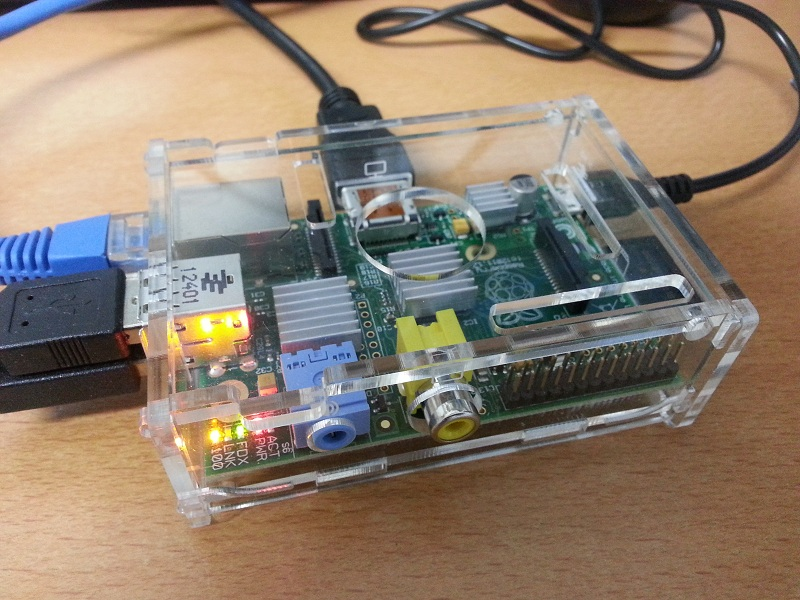
\includegraphics[width=.6\textwidth]{pic/real}
  \caption{树莓派实物图}
  \label{fig:real}
\end{figure}

图~\ref{fig:real}所示就是我们使用的树梅派。连接树梅派的还有如下一些硬件设备:
\begin{itemize}
\item SD卡一张(我们选用的是兼容树莓派的SanDisk卡 见附录~\ref{sec:sdcard})
\item HDMI高清线,VGA转接头,网线
\item 键盘鼠标
\item 电源
\end{itemize}

树莓派的物理结构如图~\ref{fig:structure}所示。

\begin{figure}
  \centering
    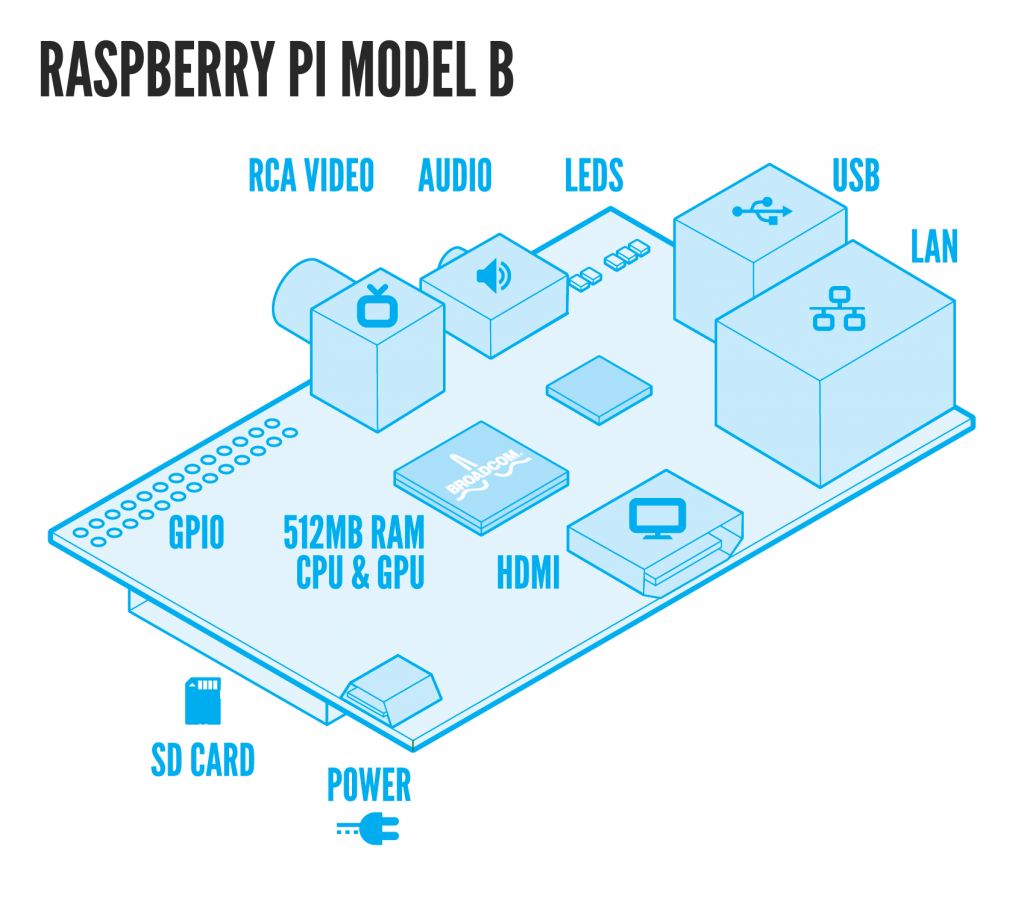
\includegraphics[width=.7\textwidth]{pic/structure}
  \caption{树莓派结构图}
  \label{fig:structure}
\end{figure}

\subsubsection{树莓派的硬件连接}

\begin{enumerate}
\item 首先将SD卡插入在树莓派上的SD卡插槽,只有一种方式插入。
\item 接下来,把usb键盘和usb鼠标插入树莓派自带的两个usb口上。
\item 确保你的显示器是开着的,接着你需要选择你的接入方式(HDMI或者DVI等等)。
\item 接着把使用树莓派的HDMI高清线接入树莓派,使用转接头接显示器的VGA插口。
\item 如果你希望你的树莓派能够联网,插入网线到网口,就在usb口旁边,如果不要联网则跳过此步。
\item 这时你应当很高兴你已经接好了所有的线以及插入了需要的SD卡,最后一部就是接入电源,树莓
  派就起来了。
\end{enumerate}

\subsubsection{登录树莓派}

\begin{enumerate}
\item 当你的树莓派已经完成启动进程后,一个登录提示符将会显示出来。默认登录树莓派的用户名
  是\verb|pi| 密码是 \verb|raspberrypi|。注意:当你输入密码的时候你看不到密码,这是linux系
  统的安全特性。
\item 在你成功登录以后,你将会看到这样的命令提示符 \verb|pi@raspberrypi~$|。
\item 要进入图形化的操作界面,输入\verb|startx|然后回车,一个漂亮的用户界面就出来了。
\end{enumerate}

\section{PYTHON模块}

\subsection{流程图}
\label{sec:desc}

\begin{figure}%[h]
  \centering
  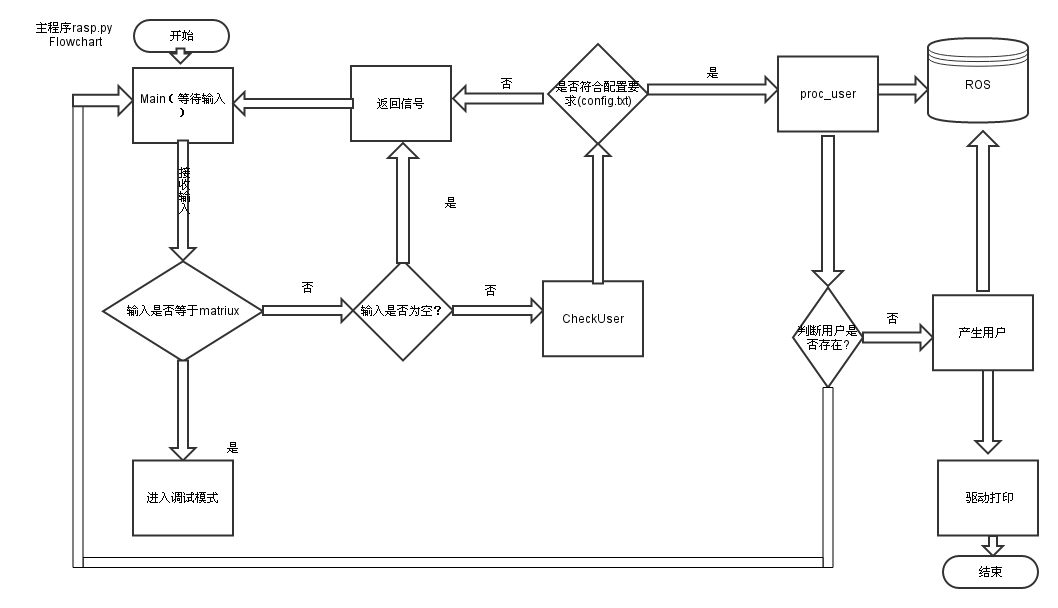
\includegraphics[width=.7\textwidth]{pic/flowchart}
  \caption{主流程图}
  \label{fig:struct}
\end{figure}

整个系统的工作流程如图\ref{fig:struct}所示。
\begin{enumerate}
\item 主程序开始$\rightarrow$进入main函数等待用户的输入(只有刷卡作为输入)。
\item 接收用户输入判断是否等于matriux(用于中断主函数等待输入的状态,便于调试)。
\item 如果输入等于预设字符串matriux,则中断监听状态,进行调试。
\item 如果输入不等于matriux,则假定输入是用户刷卡的输入。
\item 判断该输入是否为空,如果为空则返回重新等待输入。
\item 如果不为空,使用CheckUser检查用户合法性(合法性的定义在config.cfg文件中,见代码~\ref{cha:conf.cfg-1}。)
\item 经判断不符合config.cfg则返回重新等待输入,若符合要求则调用\verb|proc_user。|
\item \verb|proc_user|首先查询ROS路由器中是否已经存在该用户,若存在则踢用户下线。若不存在则
  生成新用户信息,存入ROS。
\item 存入ROS成够后调用打印机打印用户名和密码给用户上网使用。
\item 继续等待其他输入$\rightarrow$结束。
\end{enumerate}

\subsection{系统整合}
%\label{sec:integrate}

\begin{enumerate}
\item 安装PyUSB
  \begin{enumerate}
  \item 从Sourceforge\footnote{\url{http://sourceforge.net/}}上面下载最新的\verb|tarbell|
  \item \verb|unzip pyusb*.zip|
  \item \verb|cd pyusb*|
  \item \verb|python setup.py build|
  \item \verb|sudo python setup.py install|
  \end{enumerate}
\item 安装\verb|escpos|
  \begin{enumerate}
  \item \verb|wget http://python-escpos.googlecode.com/files/python-escpos-1.0.tgz|
  \item \verb|tar zxvf python-escpos-1.0.tgz|
  \item \verb|cd python-escpos-1.0|
  \item \verb|python setup.py build|
  \item \verb|sudo python setup.py install|
  \end{enumerate}
\item 安装其他软件:\verb|apt-get install python-imaging python-usb python2.7-usbtc08 python-serial|
\item PYTHON编码完成后在Raspberry Pi上测试
\item 各个程序模块已经能够在Raspberry Pi的linux系统下运行
\item 定制系统开机脚本,开机自动运行PYTHON程序
\item 测试系统稳定性
\end{enumerate}

\subsection{功能函数}

表~\ref{tab:functions}列出了程序中主要的一些函数以及函数对应的用法。

\begin{longtable}{l|l}
  \caption{函数说明}\\\hline
  函数 & 功能 \\\hline\endfirsthead
  \caption{函数说明(续)}\\\hline\endhead
  getAdminInfo & 获取admin用户的信息\\
  getNewPwd & 通过给定字符串随机构造新密码\\
  checkUser & 检查用户的合法性,通过config文件检查,返回用户名\\
  \verb|proc_user| & 写入ros数据库,产生用户名和密码\\
  getpass & termios监听程序,持续监听刷卡获得的卡号\\
  getCardNum & 刷卡后获得卡号\\
  termios.tcgetattr & 获取文件描述符\\
  termios.tcsetattr & 设置文件描述符\\
  ros.getUserlist & 获取用户列表\\
  ros.delUser & 删除用户\\
  ros.addNewUser & 添加用户\\
  rasprint.raspout & 打印输出\\
  Printer.Usb(0x04b8,0x0202) & 获取打印机标识、用于本地打印\\
  &用命令 “lsusb” 获取到当前打印机的”\\
  &Vendor ID” 和”Product ID”\\
  &假如获取到的是0x04b8:0×0202,\\
  main & 主程序\\
  \label{tab:functions}
\end{longtable}

%%% Local Variables: 
%%% mode: latex
%%% TeX-master: "../thesis"
%%% End: 
